% Version B (h16 not adopted): the one-quantity read-out as a registered variant in the appendix; main text unchanged.
\newcommand\TFaces{命題A1}
\newcommand\TLimits{定理A1}
\newcommand\TValid{定理A2}
\newcommand\TEscape{定理A3}
\newcommand\TCapture{定理A4}
\newcommand\CSep{系A1}
\section{一つの量としての読み出し（登録した変種）}
\label{sec:app_h16}
本文の読み出し$\sigma$は，支持画像と種からの2本の伝播の較正順位を掛け，2つの折で交差適合したものである．これを一つの量「画像から出たランダムウォークは支持画像と種のどちらに先に着くか」に置き換える読み出しを，開発用分割dev1での探索の後に登録し，dev2で確認し，テスト集合で構成を凍結したまま評価した（付録\ref{sec:app_hyp}）．dev2では登録した仮説がすべて成立したが，ベンチマークでは$\sigma$に及ばなかった（\tabref{h16}）．

\subsection{定義}
\label{sec:h19def}
支持画像$\mathcal{S}$，参照画像$\mathcal{R}$，較正画像$\mathcal{C}$，テスト画像$\mathcal{T}$のすべてを節点とする．ビュー$v$ごとに，各節点からコサイン類似度の上位$k_g{=}10$の節点へ重み$a^v_{ij}=\max(f_v(x_i)^{\top}f_v(x_j),0)$の辺を張って$W_v=\max(A_v,A_v^{\top})$とし，それぞれの次数の中央値で割って足した$W=\sum_vW_v/\mathrm{med}_i\,\delta^v_i$を1つのグラフとする（次数$\delta_i=\sum_jW_{ij}$，$P=D^{-1}W$）．$\mathcal{R}$，$\mathcal{C}$，$\mathcal{T}$はすべてラベルのない節点として同じ扱いを受け，グラフは節点の名札に依らない．

このグラフの上で，節点$i$に平均$1/\delta_i$の指数時間とどまり，確率$P_{ij}$で$j$へ跳ぶ連続時間のランダムウォーク$X_t$を考える．ランダムウォークはジャンプのたびに確率$1-\lambda$で，また単位時間あたり率$\gamma$で消える．支持画像と種$\hat{Q}$（\secref{seed19}）を吸収壁とし，
\begin{equation}
\begin{aligned}
h(x)&=\Pr\nolimits_x\big(\text{消える前に，}\hat{Q}\text{より先に}\mathcal{S}\text{に着く}\big)\\
&=\mathbb{E}_x\big[\lambda^{N}e^{-\gamma T};\,\tau_{\mathcal{S}}<\tau_{\hat{Q}}\big]
\end{aligned}
\label{eq:h}
\end{equation}
を画像$x$のIDらしさとする（$\tau_A$は集合$A$に初めて着く時刻，$N$と$T$はそこまでのジャンプの回数と時間）．$h$は「支持画像に着く」「種に着く」「消える」という排反な3つの行き先のうち，支持画像が最初になる確率であり，3つの確率の和は1である（付録\ref{sec:app_h19}）．$\lambda{=}1,\gamma{=}0$では調和関数~\cite{zhu2003harmonic}やランダムウォーカーによる領域分割~\cite{grady2006rw}の到達確率，一般には部分吸収ランダムウォーク~\cite{wu2012parw}の一つの形である．

\textbf{\TFaces（三つの表示）．}自由な節点を$F=V\setminus(\mathcal{S}\cup\hat{Q})$とすると，次の3つは同じ$h$を与える．(i) 確率\eqnref{h}．(ii) 連立一次方程式$(D+\gamma I-\lambda W)_{FF}\,h_F=\lambda W_{F\mathcal{S}}\mathbf{1}$（係数行列は対称正定値）．(iii) $f|_{\mathcal{S}}=1$，$f|_{\hat{Q}}=0$のもとで
\begin{equation}
\mathcal{E}(f)=\lambda\sum_{i<j}W_{ij}(f_i-f_j)^2+\sum_i\big((1-\lambda)\delta_i+\gamma\big)f_i^2
\label{eq:energy}
\end{equation}
を最小にする$f$．これは辺に伝導度$\lambda W_{ij}$，各節点と接地の間に伝導度$(1-\lambda)\delta_i+\gamma$の漏れを置いた抵抗回路で，支持画像を電位1，種を接地したときの電位である~\cite{doyle1984}（証明は付録\ref{sec:app_h19}）．

\textbf{二つの代価．}\eqnref{energy}の漏れ$(1-\lambda)\delta_i$は次数に比例するので，これだけなら$W$を定数倍しても$h$は変わらず，$h$はグラフの形（$P$）だけで決まる．漏れ$\gamma$は絶対的で，次数の小さい疎な節点ほど流れの多くを失う．1回の訪問で消えずに次へ跳ぶ確率$\rho_x=\lambda\delta_x/(\delta_x+\gamma)$は疎な節点で小さい．$h(cW;\lambda,c\gamma)=h(W;\lambda,\gamma)$なので，$\gamma$は次数の中央値に対する比$g$で置き，$h$を重みの全体の尺度に依らない量にする．

\textbf{\TLimits（二つの代価の極限）．}(i) 種がなく，$\lambda=1-\mu\varepsilon$，$\gamma=\nu\varepsilon$（$\mu,\nu\ge0$）とすると，$\varepsilon\to0$で$(1-h(x))/\varepsilon\to\mu\,\mathbb{E}_x[N_{\mathcal{S}}]+\nu\,\mathbb{E}_x[T_{\mathcal{S}}]$である（$N_{\mathcal{S}}$，$T_{\mathcal{S}}$は支持画像に着くまでの歩数と時間）．(ii) 支持画像に置いた質量を伝播させる局所・大域一貫性~\cite{zhou2004lgc}の解$u=(1-\lambda)(I-\lambda D^{-1/2}WD^{-1/2})^{-1}\mathbf{1}_{\mathcal{S}}$は，連結なグラフで$\lambda\to1$のとき$\sqrt{\boldsymbol{\delta}}$に比例する量に収束する．

\textbf{形と密度．}(i)から，代価の小さい極限で種のない$h$の順位は，支持画像に着くまでの期待費用「1歩あたり$\mu$，時間あたり$\nu$」で決まる．ランダムウォークは節点$i$に平均$1/\delta_i$とどまるので，時間は経路の疎さを，歩数はたどる近傍の段数を測る．支持画像と疎にしかつながらない未知の塊（near-OOD）は形の現象，IDから離れた疎な領域（far-OOD）は密度の現象であり，二つの代価が一本のランダムウォークの上でそれぞれを測る（\figref{toy}）．支持画像を吸収壁にしない伝播(ii)は，ランダムウォークが支持画像を通り抜けて定常分布に近づくため次数だけの量に退化するが，$h$は支持画像に着いた時点で止まる．

% 付録は1段組：模式図は浮動させず，定義の節の終わりに置く（読み出しの手順の途中に入らないように）
\par\medskip
\noindent\begin{minipage}{\linewidth}
\centering
\makeatletter\def\@captype{figure}\capwidth\hsize\ecapwidth\hsize\abovecaptionskip1mm\belowcaptionskip\z@\makeatother
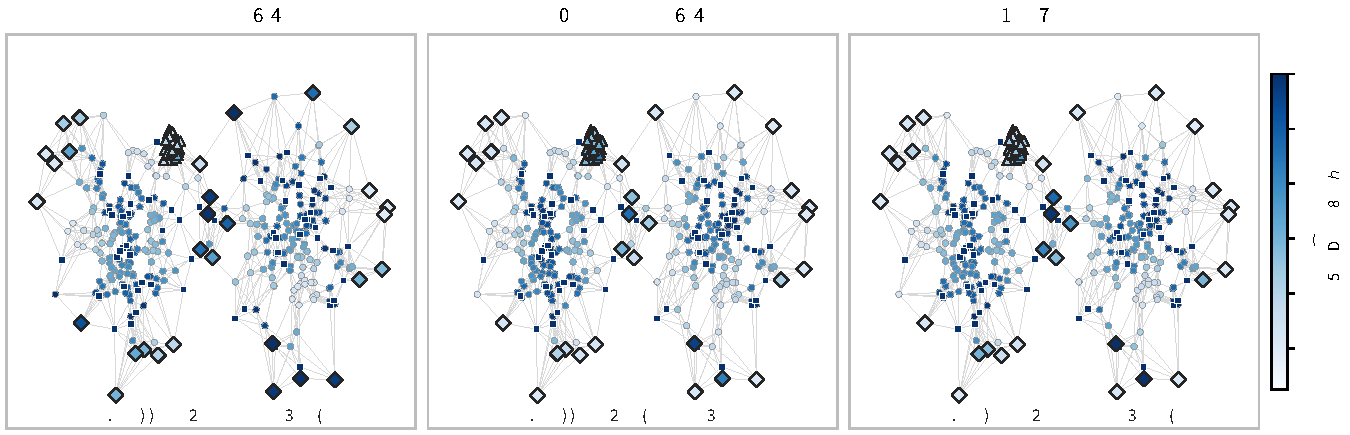
\includegraphics[width=0.86\linewidth]{figs/fig_toy19.pdf}
\caption{同じ量$h$と二つの代価（2次元の模式例；ガウス重みの対称な$k$近傍グラフ，$k{=}8$）．■は支持画像，○はIDのラベルなし画像，▲は密な未知の塊，◆は疎に散らばった未知で，色はラベルなし画像の中での$h$の順位（薄いほどOODらしい）．(a) 歩数の代価だけ（$\lambda{=}0.8$，$\gamma{=}0$）は塊を捉えるが散らばった未知を逃し，(b) 時間の代価だけ（$\lambda{=}1$，$\gamma$は次数の中央値の0.3倍）はその逆になり，(c) 二つの代価（$\lambda{=}0.8$，$\gamma$は0.03倍）は両方をIDより下に置く．種は使っていない．}
\label{fig:toy}
\end{minipage}
\par\medskip


\subsection{種と較正順位}
\label{sec:seed19}
ラベル付き画像をクラスごとに支持画像12枚，参照画像2枚，較正画像2枚に，画像に依らない位置で分ける．(1) 種のない$h$を$h^{(0)}$とし，プール$\mathcal{U}=\mathcal{C}\cup\mathcal{T}$の各画像を参照画像の中での順位$p_{\mathcal{R}}(u)=(1+|\{r\in\mathcal{R}:h^{(0)}(r)\le h^{(0)}(u)\}|)/(|\mathcal{R}|+1)$で読む．(2) $p_{\mathcal{R}}$にStorey型のBH法~\cite{benjamini1995bh,storey2002}（水準$q{=}0.2$）をかけ，棄却された画像を種$\hat{Q}\subset\mathcal{U}$とする（較正画像も候補に入る）．(3) 種を吸収壁にした$h$を解き，すべてのラベルなし画像を一歩先読みの値
\begin{equation}
s(x)=\rho_x\,(Ph)(x)=\frac{\lambda(Wh)(x)}{\delta_x+\gamma}
\label{eq:s}
\end{equation}
で採点する．種でない画像では$s=h$，種では「一歩跳んだ後に種より先に支持画像に着く確率」（自分に戻れば種に着いたとみなす）である．(4) $s$の較正画像の中での順位
\begin{equation}
p(x)=\frac{1+|\{x'\in\mathcal{C}:s(x')\le s(x)\}|}{|\mathcal{C}|+1}
\label{eq:p}
\end{equation}
を判定に，$s$を順位付けに使う．較正画像の集合は1つなので$p$は$s$の単調関数であり，二つは同点を除いて同じ順序を与える．計算は疎な正定値系2本を共役勾配法で解くだけである．

\textbf{\TValid（有効性）．}較正画像とIDのテスト画像が，他のすべての画像を所与として交換可能なら，(i) IDのテスト画像$x$について$\Pr(p(x)\le\alpha)\le\alpha$，(ii) $\{p(x)\}_{x\in\mathcal{T}}$はIDの画像の上でPRDSであり，水準$q$のBH法で選んだ集合の偽発見率は$q\,m_0/m$以下，Storey型では$q$以下である（$m_0$はIDのテスト画像の数）．(iii) さらに参照画像とプールのIDの画像が交換可能なら，種の偽発見率も$q$以下である．$s$は$\mathcal{S}$，$\mathcal{R}$と$\mathcal{U}$の画像の特徴の集まり（順序なし）だけの関数で，$\mathcal{U}$の中でどの画像を較正画像と呼ぶかに依らない．これはAdaDetect~\cite{marandon2024adadetect}の条件であり，$p$は同論文の経験$p$値である（付録\ref{sec:app_h19}）．種を$\mathcal{T}$だけから$\mathcal{C}$に対する順位で選ぶと$s$が較正画像の名札に依存して条件が崩れる．参照画像を分けて較正画像も種の候補にすることで，較正画像とテスト画像を折に分けずに保証が得られる．


\subsection{逃げる確率と捕まる確率}
\label{sec:sep19}
両側の評価は一つの関数
\begin{equation}
\varphi(\rho,a,b)=\frac{\rho\,a}{1-\rho\,(1-a-b)}\qquad(a=0\text{では}\varphi=0)
\label{eq:phi}
\end{equation}
で書ける．$\varphi$は$\rho$と$a$について増加，$b$について減少し，漏れがなければ
\begin{equation*}
\varphi(1,a,b)=\frac{a}{a+b}
\end{equation*}
である．出口$a$と出口$b$の競争に，訪問ごとの生存率$\rho$が掛かる量と読める．

\appblock
\textbf{\TEscape（逃げる確率：未知の側）．}支持画像も種も含まない節点の集合$Q$について，$Q$を初めて出る先が$z$である割引確率を$H_Q(y,z)$とすると，
\begin{equation*}
h(y)=\sum_{z\in\partial Q}H_Q(y,z)\,h(z)\qquad\text{（等式）}
\end{equation*}
であり，種でない外へ逃げる確率
\begin{equation*}
\pi_Q(y)=\sum_{z\in\partial Q\setminus\hat{Q}}H_Q(y,z)
\end{equation*}
について$h(y)\le\pi_Q(y)$である．$y\in Q$の重みのうち種でない外へ向かう割合を$e_y$，種へ向かう割合を$\zeta_y$とすると，
\begin{equation*}
\pi_Q\le\varphi\big(\max_Q\rho,\ \max_Qe,\ \min_Q\zeta\big).
\end{equation*}

\appblock
\textbf{\TCapture（捕まる確率：IDの側）．}支持画像も種も含まない節点の集合$B$について，$y\in B$の重みのうち支持画像へ向かう割合を$\omega_y$，$B$にも支持画像にも属さない節点へ向かう割合を$\eta_y$とすると，$B$を出ずに支持画像に着く確率$\kappa_B$について
\begin{equation*}
h\ge\kappa_B\ge\varphi\big(\min_B\rho,\ \min_B\omega,\ \max_B\eta\big)
\end{equation*}
である．また，すべてのラベルなし画像で
\begin{equation*}
s(x)\ge\rho_x\,\omega_x
\end{equation*}
である．

\appblock
\textbf{\CSep（分離）．}種でないテスト画像$y$が\TEscape{}の$Q$に属し，各較正画像$x'$について$\ell(x')\le s(x')$（例えば$\ell(x')=\rho_{x'}\omega_{x'}$）なら，
\begin{equation}
p(y)\le\frac{1+|\{x'\in\mathcal{C}:\ell(x')\le\pi_Q(y)\}|}{|\mathcal{C}|+1}.
\label{eq:sep}
\end{equation}
特に$\pi_Q(y)<\min_{x'\in\mathcal{C}}\ell(x')$なら$p(y)$は床$1/(|\mathcal{C}|+1)$に落ち，$y$は$\alpha\ge1/(|\mathcal{C}|+1)$のすべての水準でOODと判定される（証明は付録\ref{sec:app_h19}）．

\appblock
\textbf{読み方．}未知の塊では「種でない外への辺」と「種への辺」が競い，IDの近傍では「支持画像への辺」と「漏れる辺」が競う．同じ$\varphi$が両側を抑え，その大小が較正順位の分離\eqnref{sep}を決める．有効性（\TValid）と検知力（\TEscape{}--\CSep）は同じ量$s$についての主張である．種を増やすと$h$は単調に減り，塊のどの節点でも重みの割合$\zeta$以上が種へ向かえば，漏れがなくても逃げる確率は
\begin{equation*}
\pi_Q\le\frac{\max_Qe}{\max_Qe+\zeta}
\end{equation*}
を満たす．同じ未知クラスの画像が複数枚あるとき，種になった画像は残りの画像の重みの一部を占め，その逃げる確率を下げる．これが自己ラベル付けの効く理由である．


\subsection{結果}
\label{sec:app_h16res}
\textbf{登録と判定．}開発用分割dev1で\NHsExplNCfg{}通りの構成を探索した後，構成を1つに固定し（$\lambda{=}0.95$，$g{=}1/16$，ビューの重みを次数の中央値で割った和のグラフ，クラスあたり支持12・参照2・較正2，$q{=}0.2$，折なし），ベース検出器との積の形を選ぶdev1の規則，dev2での3つの仮説，採否の規則を登録してから実行した（付録\ref{sec:app_hyp}）．dev1の規則は積を$s_0\cdot p$に決めた（$s_0\cdot s$は$\times$TINSのfar-OODが\NHsDevOneTinsFarS\%で$\sigma$の\NHsDevOneTinsSigFar\%+0.5を超える）．dev2ではH1（near-OODの\FPR{}の差が+0.5以下）が\NHsDevTwoNearD{}，H2（far-OOD）が\NHsDevTwoFarD{}，H3（$p$の誤警報率が$\alpha{=}0.05$で0.06以下，$0.2$で0.21以下）が\NHsDevTwoFprFive{}／\NHsDevTwoFprTwenty{}とすべて成立し，登録した規則では$h$を主構成にすることになった．ただし\AUC{}は$\sigma$より低かった（\NHsDevTwoNearDAuc{} [\NHsDevTwoNearDAucLo, \NHsDevTwoNearDAucHi]，\NHsDevTwoFarDAuc{} [\NHsDevTwoFarDAucLo, \NHsDevTwoFarDAucHi]ポイント）．

\begin{table*}[htbp]
\centering
\caption{一つの量$h$（登録した構成）と本文の$\sigma$（単体，ベンチマークは6通りの抽出の平均，dev2は5通り；差は$h-\sigma$，抽出を単位とする対応のある95\% $t$区間）．$\times$TINSの$h$はdev1の規則で選んだ$s_0\cdot p$．}
\label{tab:h16}
\vspace{1.5mm}
{\fontsize{6.5pt}{7.6pt}\selectfont\renewcommand{\arraystretch}{1.0}%
\setlength{\tabcolsep}{1.7pt}\begin{tabular}{@{}lcc|cc|c@{}}
\hline
\rule[-2.0pt]{0pt}{8.6pt} & \multicolumn{2}{c|}{$\sigma$（本文）} & \multicolumn{2}{c|}{一つの量$h$} & \\
\rule[-2.0pt]{0pt}{8.6pt}設定 & \AUC & \FPR & \AUC & \FPR & \FPR{}の差 [95\%区間] \\
\hline
dev2 near（登録した確認） & 97.16 & 12.92 & 96.89 & 12.87 & -0.06 [-1.00, +0.89] \\
dev2 far（登録した確認） & 96.56 & 16.73 & 96.18 & 16.98 & +0.25 [-1.04, +1.54] \\
\hline
ImageNet-1K near-OOD & 97.94 & 11.50 & 97.18 & 13.65 & +2.14 [+1.70, +2.58] \\
ImageNet-1K far-OOD & 98.79 & 5.17 & 98.20 & 7.32 & +2.15 [+1.87, +2.42] \\
Four-OOD & 98.80 & 4.56 & 98.04 & 7.00 & +2.44 [+2.06, +2.81] \\
\hline
ImageNet-200 near-OOD & 98.17 & 9.07 & 96.57 & 8.10 & -0.97 [-1.38, -0.56] \\
ImageNet-200 far-OOD & 99.35 & 2.15 & 98.59 & 4.15 & +2.00 [+1.77, +2.23] \\
CIFAR-100 near-OOD & 99.18 & 2.90 & 98.44 & 6.42 & +3.52 [+3.17, +3.87] \\
CIFAR-100 far-OOD & 99.37 & 2.34 & 97.56 & 3.31 & +0.97 [+0.50, +1.44] \\
\hline
ImageNet-1K near-OOD $\times$TINS & 98.09 & 10.50 & 96.75 & 18.58 & +8.09 [+7.54, +8.64] \\
ImageNet-1K far-OOD $\times$TINS & 99.05 & 4.16 & 98.88 & 4.92 & +0.77 [+0.60, +0.93] \\
Four-OOD $\times$TINS & 99.09 & 3.39 & 98.97 & 3.56 & +0.18 [+0.07, +0.28] \\
\hline
\end{tabular}}%

\end{table*}

\textbf{ベンチマーク．}テスト集合では$h$は$\sigma$に及ばない（\tabref{h16}）．ImageNet-1Kの\FPR{}はnear-OODで\NHsTestNearSigFpr\%から\NHsTestNearFpr\%（差\NHsTestNearD{} [\NHsTestNearLo, \NHsTestNearHi]），far-OODで\NHsTestFarSigFpr\%から\NHsTestFarFpr\%，Four-OODで\NHsTestFourSigFpr\%から\NHsTestFourFpr\%になり，\AUC{}はそれぞれ\NHsTestNearDAuc{}，\NHsTestFarDAuc{}，\NHsTestFourDAuc{}ポイント下がる．ImageNet-200のnear-OODだけは\FPR{}が\NHsInTwoHundredNearD{}ポイント良いが\AUC{}は\NHsInTwoHundredNearDAuc{}ポイント低く，far-OODとCIFAR-100では悪い．$\times$TINS（$s_0\cdot p$）のnear-OODは\NHsTestNearTinsSigFpr\%から\NHsTestNearTinsFpr\%へ大きく悪化する．$p$の床の上ではベース検出器が未知の順序を決めるためで，本文が$\sigma$との積を取る理由（\secref{score}）と同じである．学習画像で較正した$p$の$\alpha{=}0.05$での誤警報率はImageNet-1Kで\NHsTestNearValFive{}／\NHsTestFarValFive{}／\NHsTestFourValFive{}であり，同じ較正の$\pfin$（\NHsTestNearSigValFive{}／\NHsTestFarSigValFive{}／\NHsTestFourSigValFive）より高い（較正画像とテスト画像は交換可能でない；\secref{fdp}）．再出現の格子では\NHsRecNCells{}条件のうち\NHsRecNBetter{}条件で$\sigma$より良いが，同じ未知クラスが1--2枚の\NHsRecNSingleton{}条件では平均\NHsRecSingletonMeanD{}ポイント悪い（NINCOの$c{=}64$，$r{=}1$で\NHsRecNincoCSixtyFourROne\%，$\sigma$は\NHsRecNincoCSixtyFourROneSig\%）．

\textbf{開発用分割から移らなかったこと．}dev2はdev1と同じ作り方で，far-OODの画像集合（OpenImage-O）も共通であり，dev2での非劣性はベンチマークに移らなかった．dev1の探索では，支持画像と種を吸収壁にして1歩ごとの代価だけを持たせた量はnear-OODで$\sigma$に並ぶがfar-OODで大きく劣り（\FPR{} \NHsExplAbsOneNear\%／\NHsExplAbsOneFar\%，$\sigma$は\NHsExplSigNear\%／\NHsExplSigFar\%），その原因は局所・大域一貫性の質量の次数成分にあった．次数だけをスコアにしても\AUC{}はfar-OODで\NHsExplDegAucFarVTwo\%（DINOv2），\NHsExplDegAucFarVThree\%（DINOv3）に達し，near-OODでは\NHsExplDegAucNearVTwo\%，\NHsExplDegAucNearVThree\%にとどまる．時間の代価$\gamma$はこの密度の手がかりを確率の中に戻すために入れたもので，dev1では$\sigma$に並んだ（\NHsExplFinNear\%／\NHsExplFinFar\%）．ベンチマークでは再出現のない未知とfar-OODで劣ることから，$\gamma$による密度の取り込みは本文の伝播の次数成分の代わりとして十分でないと考えられる．

\textbf{位置づけ．}以上から，本稿は登録した採否の規則に従わず，$\sigma$を主構成のまま，$h$を登録した変種として報告する．これは登録からの逸脱であり，その判断はテスト集合の値を見た後に行った．ただし「結果が良ければ本文，悪ければ付録に置く」ことは実行の前に決めていた（登録文書には書いていない；付録\ref{sec:app_hyp}）．$h$は誤警報率の保証（\TValid）と検知力（\TEscape{}--\CSep）を同じ量について述べられるが，ベンチマークでの性能は$\sigma$に及ばない．

